% Rangefinding Hardware

\chapter{Rangefinding Hardware} % Main chapter title

\label{RangefindingHardware}

\section{Wireless Communications}
At the start of the project, it was determined that a technology would need to be chosen to handle wireless communications for ranging purposes. A number of options were considered. The ideal technology would:
\begin{itemize}
	\item Be inexpensive (a per-tag cost below \$100).
	\item Have a range exceeding 5m for in-door use.
	\item Allow for at least nanosecond-precision measurements of time. Due to the speed of light, a nanosecond of error in timing calculations would lead to approximately 30cm of error, so every nanosecond is significant.
	\item Be small (easily attachable to a standard Android phone).
\end{itemize}

Bluetooth was initially considered and explored for the wireless technology of the rangefinding subsystem, but it was found to not be appropriate for the project. Appendix~\ref{BluetoothFailure} goes into some details.

\subsection{Ultra-wideband and the DWM1000}
After doing some research, the Decawave DWM1000 ultra-wideband transceiver was discovered. The chip is advertised as specifically being suited for in-door ranging applications. It uses ultra-wideband technology rather than Bluetooth, Wi-Fi, or similar technologies.

\textbf{Ultra-wideband}, in contrast to Wi-Fi and other radio technologies, occupies a large bandwidth and transmits information via high-bandwidth pulses. Ultra-wideband is suited to in-door tracking applications due to how multipath propagation, a phenomenon where signals reflect off of surfaces and thus reach the antennae via multiple paths, enhances signal strength rather than causing interference as occurs in other radio technologies. 

An in-depth look at ultra-wideband is beyond the scope of this report.

The DWM1000 is advertised as:
\begin{itemize}
	\item Able to locate objects with up to 10cm accuracy,
	\item Having a range of up to 290m,
	\item Having a data rate of up to 6.8Mb/s,
	\item And having a small physical size. 
\end{itemize}

In addition, there was an already an open source library written to use the DWM1000 with an Arduino, which would allow us to quickly prototype with the chip and ensure it would be a good choice for the project.

Because these qualities satisfied our requirements, the DWM1000 was chosen for the foundational technology of the ranging part of the project. 

\section{Design of the Hardware}
The hardware design for tags is an Arduino Pro Mini 3.3V connected to a DWM1000 over a PCB. 

\subsection{The Microcontroller}
To interface with the DWM1000, a microcontroller was needed. The Arduino Pro Mini 3.3V was chosen because:
\begin{itemize}
	\item Others had used it with the DWM1000 and had good results \cite{LPSMini}.
	\item Members of Group 20 had previous experience with programming Arduinos.
	\item It was inexpensive (\$13 before tax).
	\item It worked off of 3.3V power, which was what the DWM1000 required. This obviated the need for voltage stepping.
	\item It was capable of floating point math, which is useful for calculating ranges. As well, barely any processing power or RAM was perceived to be needed. Each microcontroller only needed to hold a small number of timestamps, so the small amount of memory and slow processor was not important. (This was later discovered to be untrue.)
	\item It had a small physical size. As tags are attached to cellphones, they must be small.
	\item Batteries would not be needed to power tags, since power could be delivered via USB from the cellphone. This further simplified the design and kept costs low, though the USB cables required to connect the Arduinos ended up being quite expensive (\$22), mostly eliminating the cost savings.
\end{itemize}

The downside of the Pro Mini was that it required a lot of soldering. 

\subsection{Anchors}
\begin{figure}
	\centering
	\includegraphics[width=\linewidth]{Figures/Anchor.jpg}
	\decoRule
	\caption{An anchor built on a breadboard using Thomas Trojer's PCB design \cite{ThotroGithub}. The DWM1000 is on the left, and the Arduino is on the right.}
	\label{fig:Anchor}
\end{figure}

The anchors made for use with this project were made on a breadboard and based on the design by Thomas Trojer in his \code{arduino-dw1000} library \cite{ThotroGithub}. A PCB design was included with this library which allowed a DWM1000 to be used with a breadboard. This PCB design was used in order to quickly prototype and determine whether the DWM1000 and Arduino would be feasible and meet the requirements for the project. Four anchors were constructed using these PCBs. An anchor can be seen in Figure~\ref{fig:Anchor}.

As anchors are assumed to be stationary, and the project is intended to be used in-doors, it was determined that the anchors could reasonably be powered via a standard electrical outlet. Designs using batteries were considered, but as the added flexibility in placement of the anchors considered to be marginal benefit (this later turned out to not be the case), and there was added complexity and maintenance required to deal with the batteries, using batteries as the power source of the anchors was not pursued.

To save costs and time, the anchors were not redesigned to be placed on a PCB, and instead remained mounted on breadboards. There was only marginal benefit to designing a PCB, as their size was mostly irrelevant and their performance would not be improved.

\subsection{Tags}
\begin{figure}
	\centering
	\includegraphics[width=\linewidth]{Figures/PCB.png}
	\decoRule
	\caption{The design for the tag PCB in EAGLE.}
	\label{fig:PCB}
\end{figure}

\begin{figure}
	\centering
	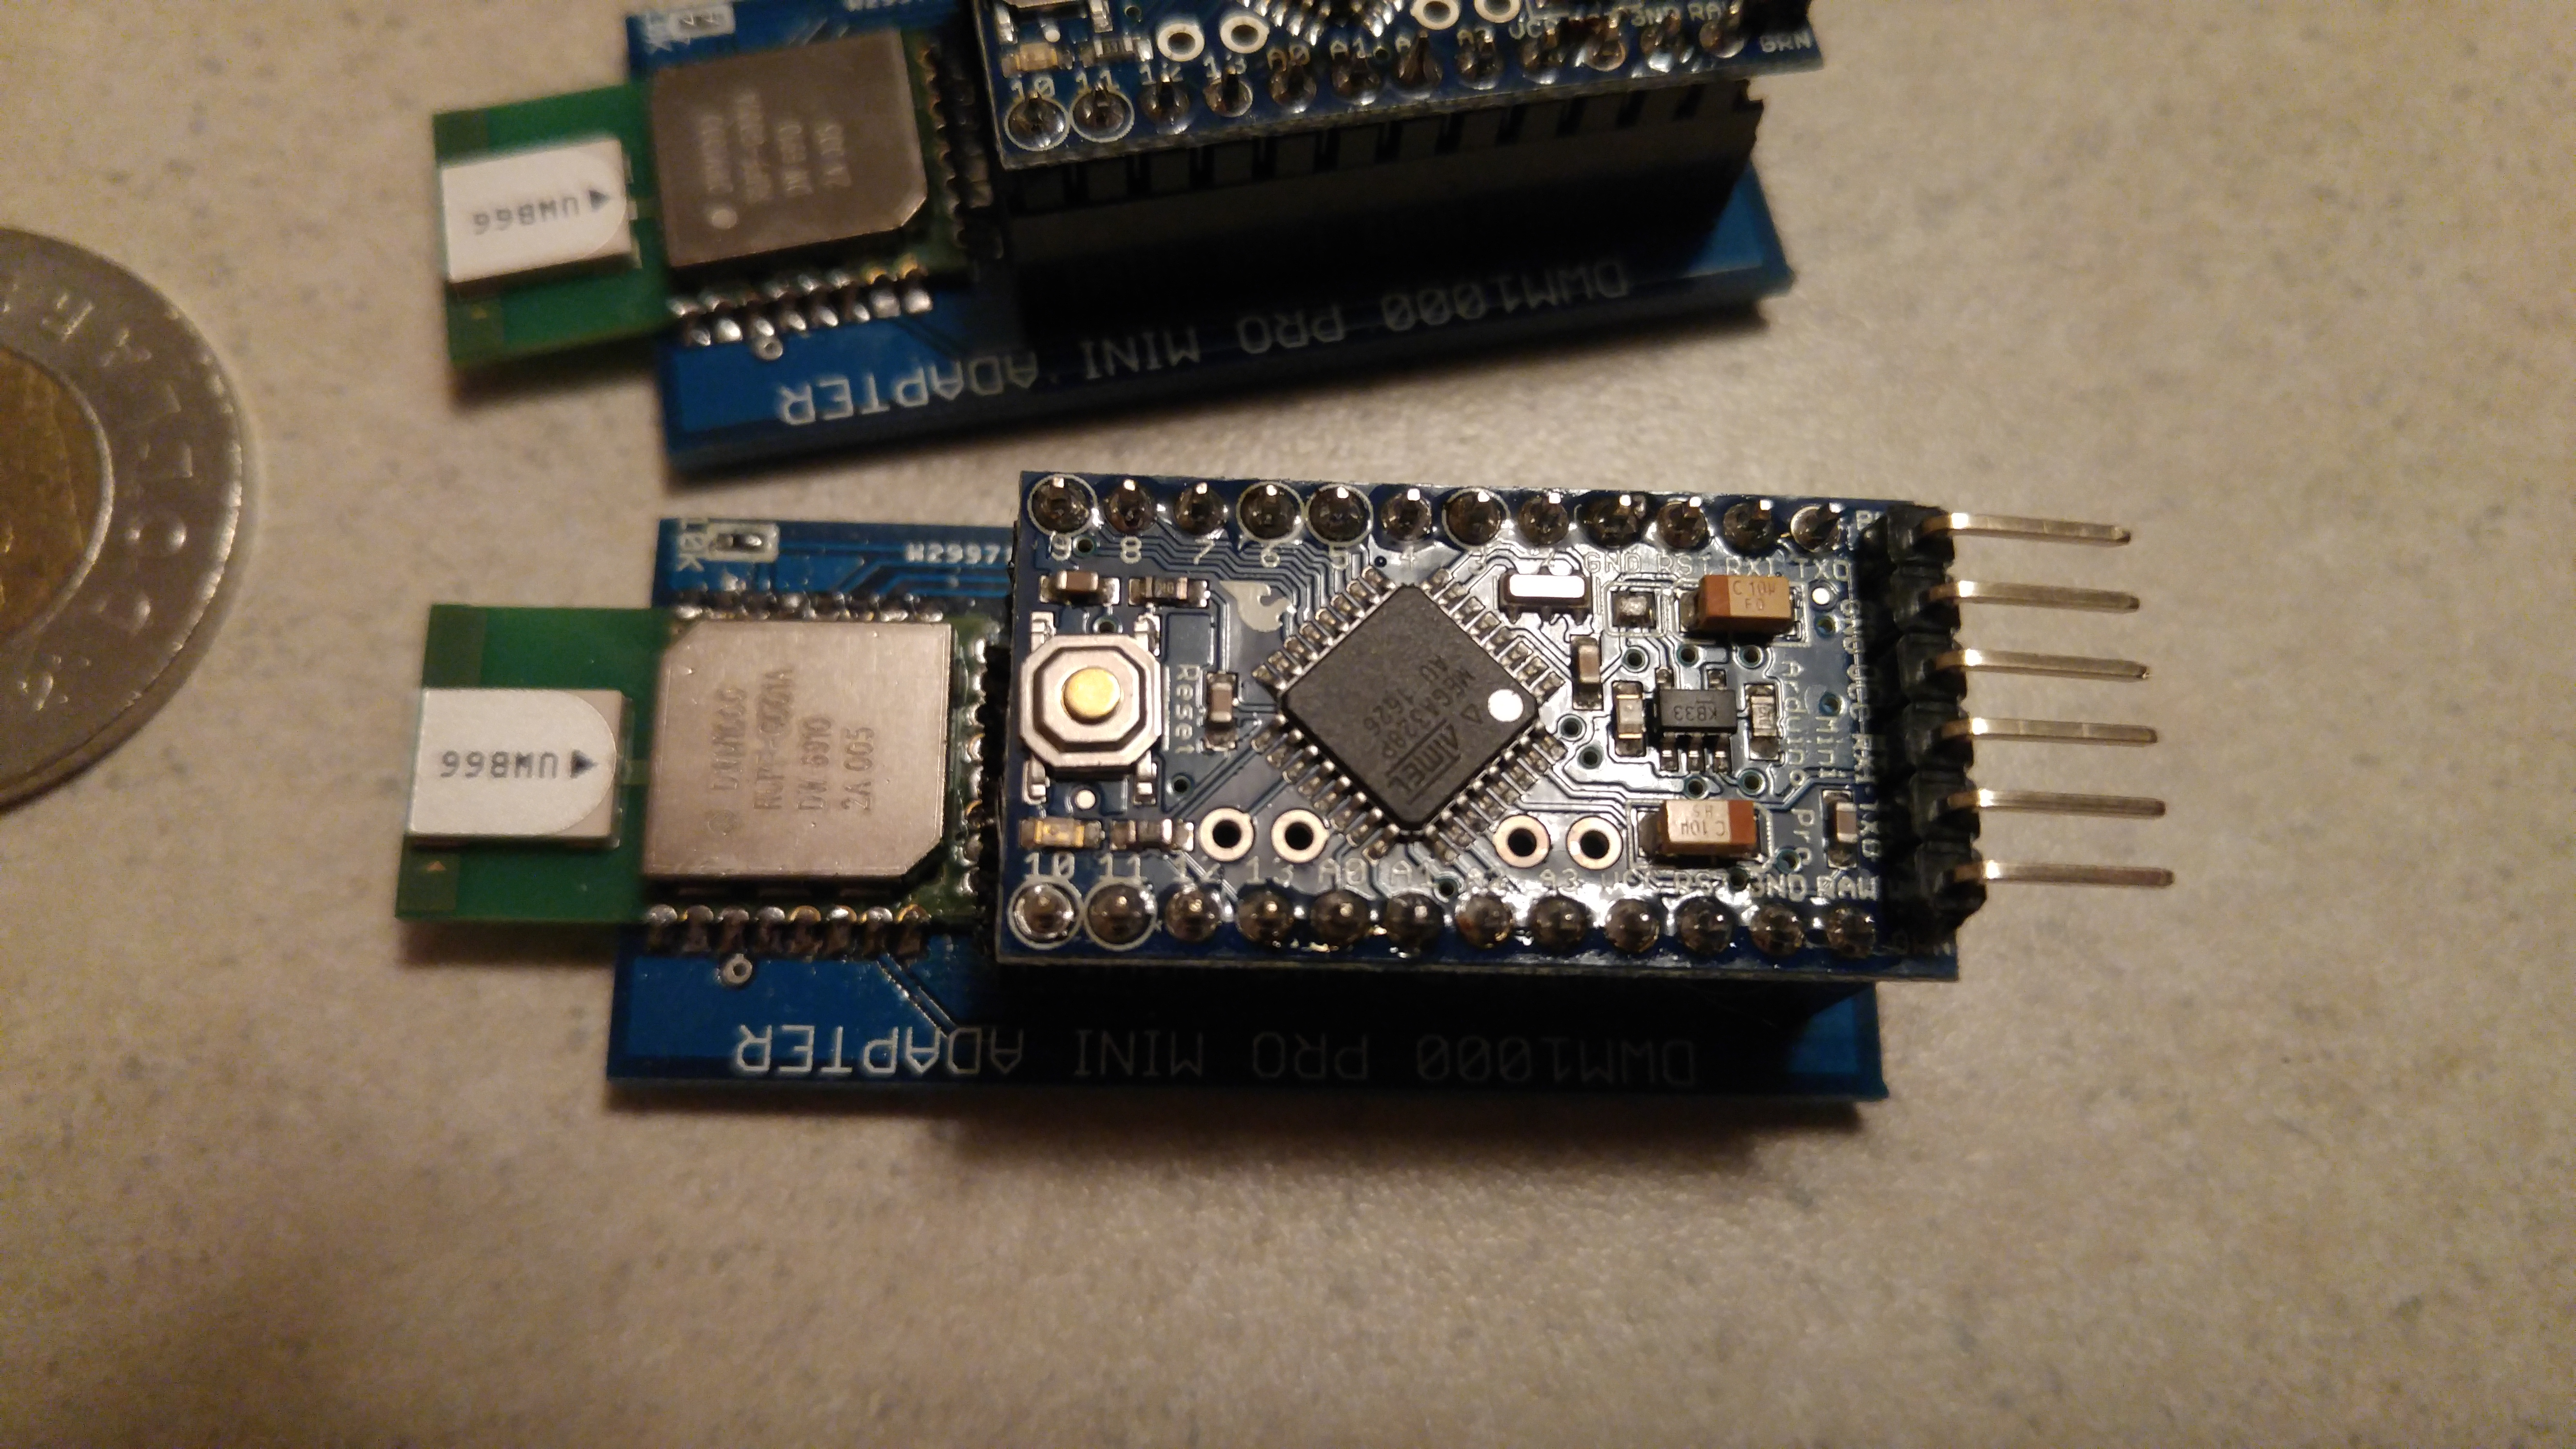
\includegraphics[width=\linewidth]{Figures/Tag.jpg}
	\decoRule
	\caption{A soldered tag.}
	\label{fig:Tag}
\end{figure}
The tags made for use with this project were required to be small enough to comfortably attach on a headset or cellphone. As the breadboards were too large, a custom PCB was designed.

Several designs were considered for the PCB connecting the Arduino and DWM1000. The most important factors were size and cost.

Several designs were considered at first:
\begin{itemize}
	\item The first idea considered was to place the Arduino and DWM on top of each other, resulting in the smallest possible size. However, the physical dimensions of the two components made this impossible. 
	\item Another possibility was to place each component on opposite sides of the PCB, but the Arduino's design demanded breakout headers to solder it into the board, which meant the PCB had to have holes drilled, which again meant that the physical dimensions of the two components interfered.
	\item Yet another idea was to make two PCBs. The Arduino would connect to a PCB above it, and that PCB would connect to a board above it with the DWM1000 soldered to it. Because it was layered, the pins connecting the layers could be arranged such that the Arduino and DWM1000 were essentially above each other, but without the locations of their pins interfering with each other. This design was abandoned because the breakout pins would add a large amount of vertical length, it was twice as expensive, and because it was much more complex to design.
	\item The final idea considered was to have the Arduino and DWM1000 just be placed next to each other on the same side of a PCB. This design was physically realizable, the least expensive, and though it was not as compact as would be ideal, it was still small enough to meet our requirements.
\end{itemize}

The last idea was chosen due to the its cheap cost, simplicity of design, and satisfactory size. 

As others who had used the DWM1000 recommended it \cite{LPSMini}, the PCB was designed so the antenna would not be on the PCB.

The PCB design was done in EAGLE and ordered from PCBWay. The PCB design can be seen in Figure~\ref{fig:PCB} and a soldered tag can be seen in Figure~\ref{fig:Tag}.

\section{Arduino Software}
The software to control the DWM1000 was written in C++ in Arduino IDE. The basic code to control the DWM1000 (handling memory address constants, communication with it via SPI, and a few high-level functions like send/receive) was available in Thomas ``thotro'' Trojer's open-source \code{arduino-dw1000} library. The library served as the foundation of the code used in this project to network the tags and anchors.

\subsection{Calculating a Delay}
\label{CalculatingADelay}
As part of the time-of-flight calculation, a timestamp is needed for when the ranging message was received and for when the reply was sent. The DWM1000 does not offer a way to automatically set the time upon transmission, but does offer the ability to set a time when a message will be transmitted in the future. If a delayed transmission is sent, the timestamp can be calculated ahead of time and then be embedded in the message.

Ideally, this delay is short. However, if the delay is too short, the Arduino will not be able to transmit the message data to the DWM1000 before the delayed timestamp is passed. This causes a silent error, and the DWM will not transmit anything. As well, the delay specified is not quite the delay at which the DWM1000 will begin transmitting, it is the delay that the DWM1000 will begin transmitting the data portion of the message. There is a ``premable'' sent before any transmission to allow the other devices in the network time to wake up and learn that a message is coming. Sending the preamble takes a relatively long time (approximately 1 microsecond per symbol in the preamble, which adds up to almost 2 ms for the preamble length chosen for this project). This was the most difficult to solve bug that was encountered in the design of the system.

The delay before a node can transmit is the sum of the:
\begin{itemize}
	\item Number of symbols in the preamble $\times$ 1\si{\micro\second} (2048 is the value used here, though the DWM offers different choices of preamble length, it is not exactly 1 \si{\micro\second} but it is very close)
	\item Time required to calculate and send the timestamp using SPI, about 1000\si{\micro\second} (empirically determined)
	\item Bytes of data to transmit $\times$ 4.5\si{\micro\second}, or 85 $\times$ number of devices in the network besides this one (empirically determined)
\end{itemize}

Adding in a fudge factor of about 200\si{\micro\second}, the delay we use in code for 6 devices is roughly 3500 \si{\micro\second}.

It is important to minimize this delay so as to increase the maximum frequency the system can update ranges at. The tradeoff of having a short preamble versus a long one is that a longer preamble takes time to send, but has a lower probability of being missed by the recipients. Tests indicated that the longest preamble, 2048 symbols, would be useful for in-door ranging due to the number of obstructions which would interfere with signals.  Shorter preambles resulted in missed messages a longer preamble could send without difficulty.

\section{Calibrating}
DWM1000s need to be calibrated to give correct distances due to the capacitance of the hardware connected to the chips, among other factors. Some of these factors are controlled for in software in the \code{arduino-dw1000} library. For a detailed overview of the possible errors and how to correct for them, the reader is advised to read the relevant sections in the DW1000 User Manual \cite{DW1000UserManual}.

The primary factor which could not be controlled for by the manufacturer, Decawave, was the antenna delay. The capacitance of the hardware the DWM1000 is hooked up to can cause nanosecond-level delays in transmission (in experiments, it was found that this could cause a meter of error or more incorrectly configured). This is a constant, and is determined empirically. The antenna delay constant for the tags is roughly the same. Good values were in the range of 16470-16500, and the antenna delay for the anchors is roughly the same and was found to be INSERT NUMBER HERE TODO.

Changing the antenna delay in the main code for easier calibration required changes to the \code{arduino-dw1000} library. A link to the code can be found in Appendix~\ref{ArduinoCode}.

\section{Results}
\label{RangefindingResults}
Results showed that the DWM1000 was close to as accurate as Decawave claimed (within 10cm). Of note, sometimes the reported ranges would glitch and be off by a meter or more. Table~\ref{tab:RangefindingAccuracy} shows the accuracy of the system. Though the accuracy of the rangefinding system was not a direct requirement of the project as a whole, the accuracy of the rangefinding system translates into accuracy of the position calculating system and thus the accuracy of the markers on the AR display.

\begin{table}
\caption{Accuracy of the rangefinding subsystem. Experiment performed with a tape measur and two tags lying on the ground. Antenna delay 16470.}
\label{tab:RangefindingAccuracy}
\centering
\begin{tabular}{c c c}
\toprule
\tabhead{Actual Distance (m)} & \tabhead{Mean Reported Distance (m)} & \tabhead{Standard Deviation (m)} \\
\midrule
0.5 & 0.62 & 0.045 \\
1 & 1.08 & 0.025 \\
2 & 2.24 & 0.03 \\
3 & 3.21 & 0.022 \\
4 & 4.22 & 0.104 \\
\bottomrule 
\end{tabular}
\end{table}

The operating frequency was close to the values predicted by the theory in Section~\ref{OperatingFrequencyAnalysis}. Predicted and actual values can be found in Table~\ref{tab:RangefindingFrequency}.

The max range between nodes was not determined due to space limitations but was at least 10m. The DWM1000 should get at least 60m if there are no obstructions \cite{DWM1000UserManual}.

\begin{table}
\caption{The frequencies of the rangefinding subsystem for various numbers of devices in the network. Experimented performed by placing an increasing number of devices in a network and calculating the duration between range reports from node 1 to node 2.}
\label{tab:RangefindingFrequency}
\centering
\begin{tabular}{c c c}
\toprule
\tabhead{Number of Devices} & \tabhead{Round Time (\si{\micro \second})} & \tabhead{Frequency (Hz)} \\
\midrule
2 & 37000 & 27 \\
3 & 58000 & 17.2 \\
4 & 86000 & 11.6 \\
5 & 93000 & 10.8 \\
6 & 156000 & 6.4 \\
7 & 170000 & 5.9 \\
\bottomrule
\end{tabular}
\end{table}
